\documentclass[birder=10pt,tikz]{standalone}
\usepackage[T1]{fontenc}
\renewcommand\rmdefault{ptm}
\usepackage{ctex,amsmath}
\usepackage{newtxmath,mathdesign}
\setmainfont{Times New Roman}
\usetikzlibrary{arrows.meta,positioning,calc,shadings,3d,patterns,fadings,mindmap}
\usepackage[most]{tcolorbox}
\begin{document}
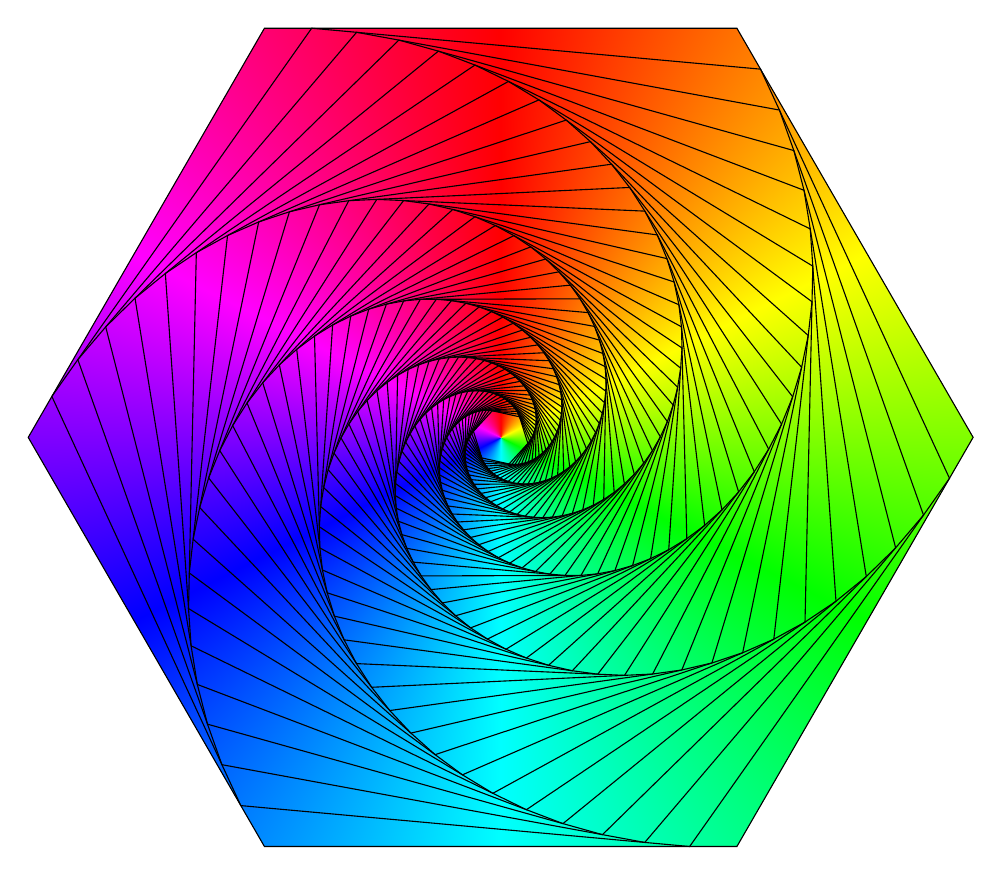
\begin{tikzpicture}
    \path[coordinate] (0,0)  coordinate(A)
                ++( 120:6cm) coordinate(B)
                ++(60:6cm) coordinate(C)
                ++(0:6cm) coordinate(D)
                ++(-60:6cm) coordinate(E)
                ++(240:6cm) coordinate(F)
                ;
    \filldraw[shading=color wheel] (A) -- (B) -- (C) --(D) -- (E) -- (F)-- cycle;
    \foreach \x in {1,...,60}{%
        \path[coordinate] coordinate(X) at (A){};
        \path[coordinate] (A) -- (B) coordinate[pos=.10](A)
                            -- (C) coordinate[pos=.10](B)
                            -- (D) coordinate[pos=.10](C)
                            -- (E) coordinate[pos=.10](D)
                             -- (F) coordinate[pos=.10](E)
                            -- (X) coordinate[pos=.10](F);
        \draw(A)--(B)--(C)-- (D) --(E) -- (F) -- cycle;
    }
\end{tikzpicture}



\end{document}
